\documentclass{article}\usepackage[]{graphicx}\usepackage[]{color}
%% maxwidth is the original width if it is less than linewidth
%% otherwise use linewidth (to make sure the graphics do not exceed the margin)
\makeatletter
\def\maxwidth{ %
  \ifdim\Gin@nat@width>\linewidth
    \linewidth
  \else
    \Gin@nat@width
  \fi
}
\makeatother

\definecolor{fgcolor}{rgb}{0.345, 0.345, 0.345}
\newcommand{\hlnum}[1]{\textcolor[rgb]{0.686,0.059,0.569}{#1}}%
\newcommand{\hlstr}[1]{\textcolor[rgb]{0.192,0.494,0.8}{#1}}%
\newcommand{\hlcom}[1]{\textcolor[rgb]{0.678,0.584,0.686}{\textit{#1}}}%
\newcommand{\hlopt}[1]{\textcolor[rgb]{0,0,0}{#1}}%
\newcommand{\hlstd}[1]{\textcolor[rgb]{0.345,0.345,0.345}{#1}}%
\newcommand{\hlkwa}[1]{\textcolor[rgb]{0.161,0.373,0.58}{\textbf{#1}}}%
\newcommand{\hlkwb}[1]{\textcolor[rgb]{0.69,0.353,0.396}{#1}}%
\newcommand{\hlkwc}[1]{\textcolor[rgb]{0.333,0.667,0.333}{#1}}%
\newcommand{\hlkwd}[1]{\textcolor[rgb]{0.737,0.353,0.396}{\textbf{#1}}}%
\let\hlipl\hlkwb

\usepackage{framed}
\makeatletter
\newenvironment{kframe}{%
 \def\at@end@of@kframe{}%
 \ifinner\ifhmode%
  \def\at@end@of@kframe{\end{minipage}}%
  \begin{minipage}{\columnwidth}%
 \fi\fi%
 \def\FrameCommand##1{\hskip\@totalleftmargin \hskip-\fboxsep
 \colorbox{shadecolor}{##1}\hskip-\fboxsep
     % There is no \\@totalrightmargin, so:
     \hskip-\linewidth \hskip-\@totalleftmargin \hskip\columnwidth}%
 \MakeFramed {\advance\hsize-\width
   \@totalleftmargin\z@ \linewidth\hsize
   \@setminipage}}%
 {\par\unskip\endMakeFramed%
 \at@end@of@kframe}
\makeatother

\definecolor{shadecolor}{rgb}{.97, .97, .97}
\definecolor{messagecolor}{rgb}{0, 0, 0}
\definecolor{warningcolor}{rgb}{1, 0, 1}
\definecolor{errorcolor}{rgb}{1, 0, 0}
\newenvironment{knitrout}{}{} % an empty environment to be redefined in TeX

\usepackage{alltt}

\usepackage{geometry}
\geometry{verbose,tmargin=1.5in,bmargin=1in,lmargin=1in,rmargin=1in}
\usepackage{fancyhdr, amsfonts, amssymb, amsmath, amsthm, MnSymbol, wasysym, bbm, mathrsfs, graphicx, listings, parskip, float, caption, booktabs}
\pagestyle{fancy}
\setlength{\parskip}{\smallskipamount}
\setlength{\parindent}{0pt}

\def\Z{\mathbb{Z}}
\def\R{\mathbb{R}}
\def\Q{\mathbb{Q}}
\def\N{\mathbb{N}}
\def\C{\mathbb{C}}
\def\P{\mathbb{P}}
\def\E{\mathbb{E}}
\def\SF{\mathscr{F}}
\def\ind{\mathbbm{1}}
\def\giv{{\,|\,}}
\def\lf{\left\lfloor}
\def\rf{\right\rfloor}
\def\lc{\left\lceil}
\def\rc{\right\rceil}
\def\eqd{ \stackrel{d}{=} }
\def\p{ \stackrel{\P}{\rightarrow} }
\def\as{ \stackrel{\text{a.s.}}{\rightarrow} }
\def\eqas{ \stackrel{\text{a.s.}}{=} }
\def\d{ \stackrel{d}{\rightarrow} }
\def\w{ \stackrel{w}{\rightarrow} }
\def\v{ \stackrel{v}{\rightarrow} }
\def\var{\text{Var}}
\newcommand{\simiid}{\overset{\textrm{i.i.d.}}{\sim}}
\newcommand{\simind}{\overset{\textrm{ind.}}{\sim}}

\setcounter{section}{-1}
\IfFileExists{upquote.sty}{\usepackage{upquote}}{}
\begin{document}

\title{STAT 243 Final Project Report}
\author{Eric Kim, Shuyu Zhao, Rui Chen, Hangyu Huang \\
Github Repository: erickim/GA}

\maketitle

\section{Installation}
In order to install the package and load it into R, please run the following. Ignore the first line if you already have \texttt{devtools}.
\begin{knitrout}
\definecolor{shadecolor}{rgb}{0.969, 0.969, 0.969}\color{fgcolor}\begin{kframe}
\begin{alltt}
\hlkwd{library}\hlstd{(devtools)}
\hlstd{devtools}\hlopt{::}\hlkwd{install_github}\hlstd{(}\hlstr{"erickim/GA"}\hlstd{)}
\hlkwd{library}\hlstd{(GA)}
\end{alltt}
\end{kframe}
\end{knitrout}


\section{Functionality and Procedure}
The Genetic algorithms (GAs) are stochastic search algorithms that mimic the process of Darwinian natural selection. GAs simulate the biological evolution, where breeding among highly fit organisms ensures desirable attributes be passed to future generations, thereby providing a set of increasingly good candidate solutions to the optimization.

The select function enables the application of genetic algorithms to problems where the decision variables are encoded as "binary".

Selection mechanism mimic the process by which parents are chosen to produce offspring. Crossover and mutation operations are used to produce offspring chromosomes from chosen parent chromosomes.

Rank-based method is applied here to prevent GAs convergence to a poor local optimum. Parents are chosen based on the rank of values of negative AIC function. Any R function, which takes as input an individual string representing a potential solution, that returns a numerical value describing its "fitness" is allowable to perform as a fitness function.

The population size is in the range of the chromosome length to two times of chromosome length. In this function, the population size is twice of chromosome length, which is the number of columns of the feature matrix.

Our solution consists of one main \texttt{select} function which will iterate over a user specified number of generations and return the most fit individual. It will make calls to helper functions, which we describe below.

\subsection{Utility Functions}
The following functions can be found in \texttt{./R/utils.R}.

\subsubsection{\texttt{initialize}}
The function \texttt{initialize} is used to create $P$ initial parents to start the genetic algorithm. In this function, we pass in the response vector and the feature matrix along with the number of candidates in the population as well as the type of regression. It will create 0-1 vectors to indicate which features are included in each candidate for the initial population, and return these vectors along with the corresponding regression fit.

\subsubsection{\texttt{crossover}}
The \texttt{crossover} function gives a mean to create two new children from two parents by swapping the segments of parents' chromosomes. We can have one point to split at, which means the chromosomes are divided into two segments and then combined with each other. We can also have multiple points to split at, and the chromosomes will combine in an alternating fashion. It will return a list with two vectors for each child.

\subsubsection{\texttt{mutate}}
The \texttt{mutate} function is used to get the child gene after mutation. In this function, we take in a mutation rate along with the child to mutate and create a 0-1 vector representing the child with each entry potentially mutated.

\subsubsection{\texttt{selection}}
\texttt{selection} is used to select parents from current generation that will produce offsprings. In this function, we provide two different methods of selection based on the probability of being chosen as a parent. The probabilities are calculated as the fitness of the individuals devided by the sum of fitness value of the whole population. The "oneprop" type randomly selects one parent based on the fitness probability and the second parent randomly with equal chance from the remaining population. The "twoprop" type will randomly select both parents based on the fitness probabilities. Note that tournament selection was one of our to-do's but we never got around to it.

\subsubsection{\texttt{fitnessRanks}}
The \texttt{fitnessRanks} function will take in a vector of fitnesses and return the ranked version. This is primarily used when we ignore original fitness values and instead use their ranks.

\subsubsection{\texttt{regFunc}}
The \texttt{regFunc} function is a nice wrapper for \texttt{lm} or \texttt{glm}. Based on the regression type and family if the type was \texttt{glm}, \texttt{regFunc} will take in a formula and the dataset and produce the appropriate fitted model.

\subsection{\texttt{select}}
The main \texttt{select} function will first initialize the first generation by calling \texttt{initialize} function. If the fitness function was left at the default of AIC, then we create a new fitness function that evaluates the negative AIC (so that higher fitness means better candidate). Otherwise we will just use the user supplied fitness function leaving it up to the user to correctly implement such a function.

We will further allow the user to specify \texttt{elitism}. If it is requested, at the start of each generation, the best candidate from the previous generation will automatically be inherited to the current generation and we will keep track of how long the most elite candidate has been carried over. We do not specify a particular convergence rule and instead allow the user to supply the maximum number of iterations as suggested by Givens/Hoeting. So the length of elitism can be used as a measure of convergence: if it is high then it means that the elite individual seems to be the best as none of the generated children are able to beat it.

Next, we start a loop to create each generation. First the fitness functions will be collected. Then the \texttt{selection} function will be called to get the new parents. \texttt{crossover} and \texttt{mutate} will then be called to generate the new children. These children along with their fitted regression model will be added to the population. We add a check where if after the first child is added our population is full at $P$, then we disregard the second child and move on.

If \texttt{elitism} was requested, we will compare the elite candidate from the previous generation to the current generation. If they were the same, then the length of elitism will be updated by 1. This will continue until the maximum number of iterations is reached at which point the variables, fitted model, fitness, fitness type, and length of elitism will be returned.

This can be summarized with the diagram in Figure 1.

\begin{figure}[H]
\centering
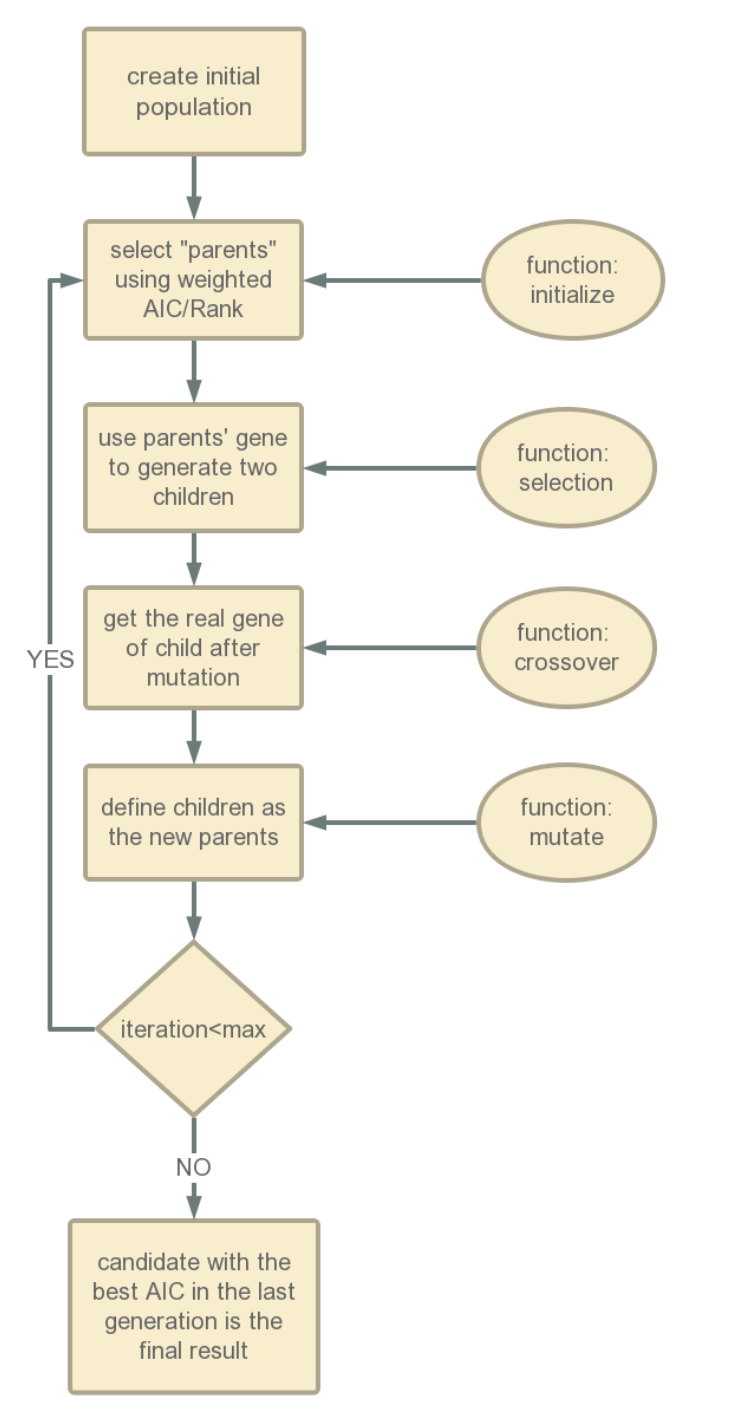
\includegraphics[width = 3in]{flow.png}
\caption{Flow chart of \texttt{select}.}
\end{figure}

\section{Testing}
We will test each of the modular pieces as well as the overall \texttt{select} function. We will make fake data as necessary to test implementation and either the \texttt{mtcars} or \texttt{Boston} datasets as we see fit for regressions. All of the following can be run using \texttt{test\_package("GA")}. There will be a couple warnings, but the tests will all pass.



\subsection{\texttt{initialize}}
Here, we look at the \texttt{mtcars} dataset. We test that when a bad argument passed in for Y or P or seed, the function will error out while when a bad argument is passed in for regType, it will default to lm and continue. We also test that when correct arguments are passed in we will get $P$ items.

\begin{knitrout}
\definecolor{shadecolor}{rgb}{0.969, 0.969, 0.969}\color{fgcolor}\begin{kframe}
\begin{alltt}
\hlstd{Y} \hlkwb{<-} \hlstd{mtcars}\hlopt{$}\hlstd{mpg}
\hlstd{X} \hlkwb{<-} \hlstd{mtcars[}\hlnum{2}\hlopt{:}\hlnum{11}\hlstd{]}
\hlstd{P} \hlkwb{=} \hlnum{2} \hlopt{*} \hlkwd{ncol}\hlstd{(X)}
\hlstd{regType} \hlkwb{=} \hlstr{'lm'}
\hlstd{family} \hlkwb{=} \hlstr{'gaussian'}
\hlstd{seed} \hlkwb{=} \hlnum{1}

\hlkwd{test_that}\hlstd{(}\hlstr{"input is invalid"}\hlstd{,\{}
  \hlcom{# Y is not valid}
  \hlkwd{expect_error}\hlstd{(}\hlkwd{initialize}\hlstd{(}\hlkwc{Y} \hlstd{=} \hlstr{"a"}\hlstd{,} \hlkwc{X} \hlstd{= X,} \hlkwc{P} \hlstd{= P,} \hlkwc{regType} \hlstd{= regType,}
                          \hlkwc{family} \hlstd{= family,} \hlkwc{seed} \hlstd{= seed))}
  \hlcom{# P needs to be a numeric}
  \hlkwd{expect_error}\hlstd{(}\hlkwd{initialize}\hlstd{(}\hlkwc{Y} \hlstd{= Y,} \hlkwc{X} \hlstd{= X,} \hlkwc{P} \hlstd{=} \hlstr{"a"}\hlstd{,} \hlkwc{regType} \hlstd{= regType,}
                          \hlkwc{family} \hlstd{= family,} \hlkwc{seed} \hlstd{= seed))}
  \hlcom{# if bad regType, it will auto default to 'lm'}
  \hlkwd{expect_is}\hlstd{(}\hlkwd{initialize}\hlstd{(}\hlkwc{Y} \hlstd{= Y,} \hlkwc{X} \hlstd{= X,} \hlkwc{P} \hlstd{= P,} \hlkwc{regType} \hlstd{=} \hlnum{1}\hlstd{,}
                       \hlkwc{family} \hlstd{= family,} \hlkwc{seed} \hlstd{= seed),} \hlstr{"list"}\hlstd{)}
  \hlkwd{expect_is}\hlstd{(}\hlkwd{initialize}\hlstd{(}\hlkwc{Y} \hlstd{= Y,} \hlkwc{X} \hlstd{= X,} \hlkwc{P} \hlstd{= P,} \hlkwc{regType} \hlstd{= P,}
                       \hlkwc{family} \hlstd{=} \hlnum{1}\hlstd{,} \hlkwc{seed} \hlstd{= seed),} \hlstr{"list"}\hlstd{)}
  \hlkwd{expect_error}\hlstd{(}\hlkwd{initialize}\hlstd{(}\hlkwc{Y} \hlstd{= Y,} \hlkwc{X} \hlstd{= X,} \hlkwc{P} \hlstd{= P,} \hlkwc{regType} \hlstd{= regType,}
                          \hlkwc{family} \hlstd{= family,} \hlkwc{seed} \hlstd{=} \hlstr{"a"}\hlstd{))}
  \hlkwd{expect_equal}\hlstd{(}\hlkwd{length}\hlstd{(}\hlkwd{initialize}\hlstd{(Y, X, P, regType, family, seed)),}
               \hlnum{2} \hlopt{*} \hlkwd{ncol}\hlstd{(X) )}
\hlstd{\})}
\end{alltt}
\end{kframe}
\end{knitrout}

\subsection{\texttt{crossover}}
Here we test when bad inputs are put into \texttt{crossover}. It will either throw an error or print a message and return NA. We also create some fake data just to test that the crossover operation actually works.

\begin{knitrout}
\definecolor{shadecolor}{rgb}{0.969, 0.969, 0.969}\color{fgcolor}\begin{kframe}
\begin{alltt}
\hlkwd{test_that}\hlstd{(}\hlstr{"input is not valid"}\hlstd{, \{}
  \hlcom{# incorrect inputs are caught}
  \hlkwd{expect_equal}\hlstd{(}\hlkwd{crossover}\hlstd{(}\hlkwd{c}\hlstd{(}\hlnum{2}\hlstd{,}\hlnum{0}\hlstd{),}\hlnum{1}\hlstd{),} \hlnum{NA}\hlstd{)}
  \hlcom{# invalid crossover type}
  \hlkwd{expect_error}\hlstd{(}\hlkwd{crossover}\hlstd{(}\hlnum{1}\hlstd{,} \hlnum{1}\hlstd{,} \hlkwc{type} \hlstd{=} \hlstr{"abc"}\hlstd{))}
\hlstd{\})}
\hlcom{# create some fake data to test crossover}
\hlstd{parent1} \hlkwb{<-} \hlkwd{rbinom}\hlstd{(}\hlnum{20}\hlstd{,} \hlnum{1}\hlstd{,} \hlnum{0.5}\hlstd{)}
\hlstd{parent2} \hlkwb{<-} \hlkwd{rbinom}\hlstd{(}\hlnum{20}\hlstd{,} \hlnum{1}\hlstd{,} \hlnum{0.5}\hlstd{)}
\hlstd{result1} \hlkwb{<-} \hlkwd{crossover}\hlstd{(parent1, parent2,} \hlkwc{type} \hlstd{=} \hlstr{"single"}\hlstd{,} \hlkwc{num_splits} \hlstd{=} \hlnum{1}\hlstd{)}
\hlstd{result2} \hlkwb{<-} \hlkwd{crossover}\hlstd{(parent1, parent2,} \hlkwc{type} \hlstd{=} \hlstr{"multiple"}\hlstd{,} \hlkwc{num_splits} \hlstd{=} \hlnum{5}\hlstd{)}
\hlkwd{test_that}\hlstd{(}\hlstr{"ouput is not expected"}\hlstd{, \{}
  \hlcom{# makes sure we get correct outputs for single splits}
  \hlkwd{expect_equal}\hlstd{(}\hlkwd{length}\hlstd{(result1}\hlopt{$}\hlstd{child1),} \hlnum{20}\hlstd{)}
  \hlkwd{expect_equal}\hlstd{(}\hlkwd{length}\hlstd{(result1}\hlopt{$}\hlstd{child2),} \hlnum{20}\hlstd{)}
  \hlkwd{expect_false}\hlstd{(}\hlkwd{any}\hlstd{(result1}\hlopt{$}\hlstd{child1} \hlopt{!=} \hlnum{0} \hlopt{&} \hlstd{result1}\hlopt{$}\hlstd{child1} \hlopt{!=} \hlnum{1}\hlstd{))}
  \hlkwd{expect_false}\hlstd{(}\hlkwd{any}\hlstd{(result1}\hlopt{$}\hlstd{child2} \hlopt{!=} \hlnum{0} \hlopt{&} \hlstd{result1}\hlopt{$}\hlstd{child2} \hlopt{!=} \hlnum{1}\hlstd{))}
  \hlcom{# makes sure we get correct outputs for multiple splits}
  \hlkwd{expect_equal}\hlstd{(}\hlkwd{length}\hlstd{(result2}\hlopt{$}\hlstd{child1),} \hlnum{20}\hlstd{)}
  \hlkwd{expect_equal}\hlstd{(}\hlkwd{length}\hlstd{(result2}\hlopt{$}\hlstd{child2),} \hlnum{20}\hlstd{)}
  \hlkwd{expect_false}\hlstd{(}\hlkwd{any}\hlstd{(result2}\hlopt{$}\hlstd{child1} \hlopt{!=} \hlnum{0} \hlopt{&} \hlstd{result2}\hlopt{$}\hlstd{child1} \hlopt{!=} \hlnum{1}\hlstd{))}
  \hlkwd{expect_false}\hlstd{(}\hlkwd{any}\hlstd{(result2}\hlopt{$}\hlstd{child2} \hlopt{!=} \hlnum{0} \hlopt{&} \hlstd{result2}\hlopt{$}\hlstd{child2} \hlopt{!=} \hlnum{1}\hlstd{))}
\hlstd{\})}
\end{alltt}
\end{kframe}
\end{knitrout}

\subsection{\texttt{mutate}}
Here, we test that bad inputs for \texttt{mutate} will error out. For correct inputs, we just check that the output is of expected length.

\begin{knitrout}
\definecolor{shadecolor}{rgb}{0.969, 0.969, 0.969}\color{fgcolor}\begin{kframe}
\begin{alltt}
\hlstd{rate}\hlkwb{<-}\hlnum{0.2}
\hlstd{offspring}\hlkwb{<-}\hlkwd{c}\hlstd{(}\hlnum{1}\hlstd{,}\hlnum{1}\hlstd{,}\hlnum{1}\hlstd{,}\hlnum{1}\hlstd{,}\hlnum{0}\hlstd{,}\hlnum{0}\hlstd{,}\hlnum{0}\hlstd{,}\hlnum{0}\hlstd{)}

\hlkwd{mutate}\hlstd{(rate, offspring)}
\end{alltt}
\begin{verbatim}
## [1] 1 1 1 0 0 1 0 0
\end{verbatim}
\begin{alltt}
\hlkwd{test_that}\hlstd{(}\hlstr{"input is invalid"}\hlstd{,\{}
  \hlkwd{expect_error}\hlstd{(}\hlkwd{mutate}\hlstd{(}\hlstr{"a"}\hlstd{, offspring))}
  \hlkwd{expect_error}\hlstd{(}\hlkwd{mutate}\hlstd{(}\hlnum{2}\hlstd{, offspring))}
  \hlkwd{expect_equal}\hlstd{(}\hlkwd{length}\hlstd{(}\hlkwd{mutate}\hlstd{(rate, offspring)),} \hlkwd{length}\hlstd{(offspring))}
\hlstd{\})}
\end{alltt}
\end{kframe}
\end{knitrout}

\subsection{\texttt{selection}}
Here we test that when bad fitnesses are passes as arguments, we will just get an NA. We also test that when we pass in fine values for the type it will work as expected while if we pass in bad arguments, it will default to ``twoprop'' and continue.

\begin{knitrout}
\definecolor{shadecolor}{rgb}{0.969, 0.969, 0.969}\color{fgcolor}\begin{kframe}
\begin{alltt}
\hlkwd{test_that}\hlstd{(}\hlstr{"Test if the input of selection is valid"}\hlstd{, \{}
  \hlkwd{expect_equal}\hlstd{(}\hlkwd{selection}\hlstd{(}\hlstr{"oneprop"}\hlstd{,}  \hlkwd{c}\hlstd{(}\hlstr{"a"}\hlstd{,}\hlstr{"a"}\hlstd{,}\hlstr{"a"}\hlstd{,}\hlstr{"a"}\hlstd{,}\hlstr{"a"}\hlstd{)),} \hlnum{NA}\hlstd{)}
  \hlkwd{expect_equal}\hlstd{(}\hlkwd{selection}\hlstd{(}\hlstr{"oneprop"}\hlstd{,}  \hlnum{2}\hlstd{),} \hlnum{NA}\hlstd{)}
  \hlkwd{expect_equal}\hlstd{(}\hlkwd{selection}\hlstd{(}\hlstr{"twoprop"}\hlstd{,} \hlkwd{c}\hlstd{(}\hlnum{2}\hlstd{,}\hlnum{3}\hlstd{,} \hlstr{"w"} \hlstd{,} \hlstr{"w"}\hlstd{)),} \hlnum{NA}\hlstd{)}
  \hlkwd{expect_equal}\hlstd{(}\hlkwd{selection}\hlstd{(}\hlstr{"twoprop"}\hlstd{,} \hlnum{2}\hlstd{),} \hlnum{NA}\hlstd{)}

\hlstd{\})}

\hlkwd{test_that}\hlstd{(}\hlstr{"Test if the output of selection is valid"}\hlstd{, \{}
  \hlkwd{expect_equal}\hlstd{(}\hlkwd{length}\hlstd{(}\hlkwd{selection}\hlstd{(}\hlstr{"oneprop"}\hlstd{,} \hlkwd{c}\hlstd{(}\hlnum{0.9}\hlstd{,}\hlnum{1.5}\hlstd{,}\hlnum{3.3}\hlstd{,}\hlnum{2.2}\hlstd{))),} \hlnum{2}\hlstd{)}
  \hlkwd{expect_equal}\hlstd{(}\hlkwd{length}\hlstd{(}\hlkwd{selection}\hlstd{(}\hlstr{"twoprop"}\hlstd{,} \hlkwd{c}\hlstd{(}\hlnum{0.9}\hlstd{,} \hlnum{1.5}\hlstd{,} \hlnum{3.3}\hlstd{,} \hlnum{2.2}\hlstd{))),} \hlnum{2}\hlstd{)}
  \hlkwd{expect_equal}\hlstd{(}\hlkwd{length}\hlstd{(}\hlkwd{selection}\hlstd{(}\hlstr{"hehehe"}\hlstd{,} \hlkwd{c}\hlstd{(}\hlnum{0.9}\hlstd{,} \hlnum{1.5}\hlstd{,} \hlnum{3.3}\hlstd{,} \hlnum{2.2}\hlstd{))),} \hlnum{2}\hlstd{)}
  \hlkwd{expect_true}\hlstd{(}\hlkwd{is.numeric}\hlstd{(}\hlkwd{selection}\hlstd{(}\hlstr{"oneprop"}\hlstd{,} \hlkwd{c}\hlstd{(}\hlnum{0.9}\hlstd{,} \hlnum{1.5}\hlstd{,} \hlnum{3.3}\hlstd{,} \hlnum{2.2}\hlstd{))))}
  \hlkwd{expect_true}\hlstd{(}\hlkwd{is.numeric}\hlstd{(}\hlkwd{selection}\hlstd{(}\hlstr{"twoprop"}\hlstd{,} \hlkwd{c}\hlstd{(}\hlnum{0.9}\hlstd{,}\hlnum{0.6}\hlstd{,}\hlnum{0.1}\hlstd{,}\hlnum{1.1}\hlstd{))))}
\hlstd{\})}
\end{alltt}
\end{kframe}
\end{knitrout}

\subsection{\texttt{fitnessRanks}}
Here, we just check that the \texttt{fitnessRanks} function is ranking properly and that it will error out if a bad argument is passed.
\begin{knitrout}
\definecolor{shadecolor}{rgb}{0.969, 0.969, 0.969}\color{fgcolor}\begin{kframe}
\begin{alltt}
\hlstd{fitness} \hlkwb{<-} \hlnum{1}\hlopt{:}\hlnum{10}
\hlkwd{fitnessRanks}\hlstd{(fitness)}
\end{alltt}
\begin{verbatim}
##  [1] 0.01818182 0.03636364 0.05454545 0.07272727 0.09090909 0.10909091
##  [7] 0.12727273 0.14545455 0.16363636 0.18181818
\end{verbatim}
\begin{alltt}
\hlkwd{test_that}\hlstd{(}\hlstr{"input is invalid"}\hlstd{,\{}
  \hlkwd{expect_equal}\hlstd{(}\hlkwd{fitnessRanks}\hlstd{(}\hlstr{"a"}\hlstd{),} \hlnum{NA}\hlstd{)}
  \hlkwd{expect_equal}\hlstd{(}\hlkwd{length}\hlstd{(}\hlkwd{fitnessRanks}\hlstd{(fitness)),}\hlkwd{length}\hlstd{(fitness))}
\hlstd{\})}
\end{alltt}
\end{kframe}
\end{knitrout}

\subsection{\texttt{regType}}
Here we test that the \texttt{regType} will perform the proper regression and we use the Boston crimes dataset from the \texttt{MASS} package to fit the model.
\begin{knitrout}
\definecolor{shadecolor}{rgb}{0.969, 0.969, 0.969}\color{fgcolor}\begin{kframe}
\begin{alltt}
\hlkwd{library}\hlstd{(MASS)}
\hlcom{# use the Boston crime dataset to check that the regression function wrapper}
\hlcom{# works as it should}
\hlstd{boston.crim} \hlkwb{=} \hlstd{Boston}\hlopt{$}\hlstd{crim}
\hlkwd{test_that}\hlstd{(}\hlstr{"Test if the output of regFunc is valid"}\hlstd{,\{}
  \hlkwd{expect_equal}\hlstd{(}\hlkwd{regFunc}\hlstd{(}\hlstr{"lm"}\hlstd{,}
                       \hlstr{"gaussian"}\hlstd{,}
                       \hlstd{boston.crim} \hlopt{~}\hlstd{.,}
                       \hlstd{Boston[,}\hlopt{-}\hlnum{1}\hlstd{])}\hlopt{$}\hlstd{Coefficients,}
               \hlkwd{lm}\hlstd{(crim}\hlopt{~}\hlstd{.,} \hlkwc{data} \hlstd{= Boston)}\hlopt{$}\hlstd{Coefficients)}
  \hlkwd{expect_equal}\hlstd{(}\hlkwd{regFunc}\hlstd{(}\hlstr{"glm"}\hlstd{,}
                       \hlstr{"gaussian"}\hlstd{,}
                       \hlstd{boston.crim} \hlopt{~}\hlstd{., Boston[,}\hlopt{-}\hlnum{1}\hlstd{])}\hlopt{$}\hlstd{Coefficients,}
               \hlkwd{glm}\hlstd{(crim}\hlopt{~}\hlstd{.,} \hlkwc{data} \hlstd{= Boston,} \hlkwc{family} \hlstd{=} \hlstr{"gaussian"}\hlstd{)}\hlopt{$}\hlstd{Coefficients)}
\hlstd{\})}
\end{alltt}
\end{kframe}
\end{knitrout}

\subsection{\texttt{select} with \texttt{Boston}}
To test whether our implementation of \texttt{select} is correct, we use the \texttt{Boston} dataset again. From the \texttt{leaps} package, we use the \texttt{regsubsets} function to perform a best subset search for all models with 1 through 13 features (13 being the maximum number of said features). We find the best AIC for these 13 best models and compare it to the final output of the \texttt{select}. We just test that both AIC's are relatively close to each other (they turn out to be the same as they picked the same models).

\begin{knitrout}
\definecolor{shadecolor}{rgb}{0.969, 0.969, 0.969}\color{fgcolor}\begin{kframe}
\begin{alltt}
\hlcom{# do a best subsets selection first}
\hlstd{bostSubsets} \hlkwb{<-} \hlkwd{regsubsets}\hlstd{(crim} \hlopt{~} \hlstd{.,} \hlkwc{data} \hlstd{= Boston,} \hlkwc{nvmax} \hlstd{=} \hlnum{13}\hlstd{)}
\hlstd{bostSubsetsWhich} \hlkwb{<-} \hlkwd{summary}\hlstd{(bostSubsets)}\hlopt{$}\hlstd{which}
\hlstd{bostSubsetsAIC} \hlkwb{<-} \hlkwd{c}\hlstd{()}

\hlkwa{for} \hlstd{(i} \hlkwa{in} \hlnum{1}\hlopt{:}\hlnum{13}\hlstd{) \{}
  \hlstd{bostSubsetsAIC} \hlkwb{<-} \hlkwd{c}\hlstd{(bostSubsetsAIC,}
                    \hlkwd{AIC}\hlstd{(}\hlkwd{glm}\hlstd{(crim} \hlopt{~} \hlstd{.,}
                            \hlkwc{data} \hlstd{= Boston[}\hlkwd{c}\hlstd{(}\hlnum{TRUE}\hlstd{,}
                                          \hlstd{bostSubsetsWhich[i,}\hlopt{-}\hlnum{1}\hlstd{])])))}
\hlstd{\}}

\hlcom{# maxIter = 50 because the dataset isn't too big}
\hlstd{bostGA} \hlkwb{<-} \hlkwd{select}\hlstd{(Boston}\hlopt{$}\hlstd{crim, Boston[,}\hlopt{-}\hlnum{1}\hlstd{],} \hlkwc{regType} \hlstd{=} \hlstr{"lm"}\hlstd{,} \hlkwc{maxIter} \hlstd{=} \hlnum{50}\hlstd{)}
\hlkwd{min}\hlstd{(bostSubsetsAIC)}
\end{alltt}
\begin{verbatim}
## [1] 3329.8
\end{verbatim}
\begin{alltt}
\hlkwd{test_that}\hlstd{(}\hlstr{"`select` comes close to the best subset selection"}\hlstd{, \{}
  \hlkwd{expect_equal}\hlstd{(}\hlopt{-}\hlnum{1}\hlopt{*}\hlstd{bostGA}\hlopt{$}\hlstd{fitness,} \hlkwd{min}\hlstd{(bostSubsetsAIC),}
               \hlkwc{tolerance} \hlstd{=} \hlkwd{min}\hlstd{(bostSubsetsAIC)}\hlopt{/}\hlnum{1e5}\hlstd{)}
\hlstd{\})}

\hlcom{# compare the selected variables}
\hlkwd{which}\hlstd{(bostGA}\hlopt{$}\hlstd{variables} \hlopt{==} \hlnum{1}\hlstd{)}
\end{alltt}
\begin{verbatim}
## [1]  1  4  7  8 10 11 12 13
\end{verbatim}
\begin{alltt}
\hlkwd{which}\hlstd{(bostSubsetsWhich[}\hlkwd{which.min}\hlstd{(bostSubsetsAIC),}\hlopt{-}\hlnum{1}\hlstd{])}
\end{alltt}
\begin{verbatim}
##      zn     nox     dis     rad ptratio   black   lstat    medv 
##       1       4       7       8      10      11      12      13
\end{verbatim}
\end{kframe}
\end{knitrout}

\subsection{\texttt{select} with \texttt{swiss}}
We do the same procedure as above except with the Swiss Fertility and Socioeconomic Indicators dataset, \texttt{swiss}, in the ``datasets'' package and has 47 observations on 6 variables. We regressed Fertility on other aspects to find the influencing factors of Swiss Fertility and try different values of maxIter. It seems that we needed more than 5 iterations but no more than 10 so for these small datasets, convergence is relatively quick as expected.
\begin{knitrout}
\definecolor{shadecolor}{rgb}{0.969, 0.969, 0.969}\color{fgcolor}\begin{kframe}
\begin{alltt}
\hlcom{#Swiss Fertility and Socioeconomic Indicators (1888) Data}
\hlstd{Y} \hlkwb{<-} \hlstd{swiss}\hlopt{$}\hlstd{Fertility}
\hlstd{X} \hlkwb{<-} \hlstd{swiss[,}\hlopt{-}\hlnum{1}\hlstd{]}

\hlcom{#use select function to select variables}
\hlstd{GASelect5} \hlkwb{<-} \hlkwd{select}\hlstd{(Y,X,} \hlkwc{maxIter} \hlstd{=} \hlnum{5}\hlstd{)}
\hlstd{GASelect10} \hlkwb{<-} \hlkwd{select}\hlstd{(Y,X,} \hlkwc{maxIter} \hlstd{=} \hlnum{10}\hlstd{)}
\hlstd{GASelect15} \hlkwb{<-} \hlkwd{select}\hlstd{(Y,X,} \hlkwc{maxIter} \hlstd{=} \hlnum{15}\hlstd{)}
\hlstd{GASelect25} \hlkwb{<-} \hlkwd{select}\hlstd{(Y,X,} \hlkwc{maxIter} \hlstd{=} \hlnum{25}\hlstd{)}
\hlstd{GASelect50} \hlkwb{<-} \hlkwd{select}\hlstd{(Y,X,} \hlkwc{maxIter} \hlstd{=} \hlnum{50}\hlstd{)}

\hlcom{#use regsubsets to select variables}
\hlstd{testBest} \hlkwb{<-} \hlkwd{regsubsets}\hlstd{(Y} \hlopt{~} \hlstd{.,} \hlkwc{data} \hlstd{= X,} \hlkwc{nvmax} \hlstd{=} \hlnum{5}\hlstd{)}
\hlstd{testBestWhich} \hlkwb{<-} \hlkwd{summary}\hlstd{(testBest)}\hlopt{$}\hlstd{which}
\hlstd{testBestAIC} \hlkwb{<-} \hlkwd{c}\hlstd{()}
\hlkwa{for} \hlstd{(i} \hlkwa{in} \hlnum{1}\hlopt{:}\hlnum{5}\hlstd{) \{}
  \hlstd{testBestAIC} \hlkwb{<-} \hlkwd{c}\hlstd{(testBestAIC,}
                   \hlkwd{AIC}\hlstd{(}\hlkwd{glm}\hlstd{(Y} \hlopt{~} \hlstd{.,}
                          \hlkwc{data} \hlstd{= X[testBestWhich[i,}\hlopt{-}\hlnum{1}\hlstd{]])))}
\hlstd{\}}

\hlcom{# compare the selected variables (not using testthat)}
\hlkwd{which}\hlstd{(GASelect5}\hlopt{$}\hlstd{variables} \hlopt{==} \hlnum{1}\hlstd{)}
\end{alltt}
\begin{verbatim}
## [1] 1 2 3 4 5
\end{verbatim}
\begin{alltt}
\hlkwd{which}\hlstd{(GASelect10}\hlopt{$}\hlstd{variables} \hlopt{==} \hlnum{1}\hlstd{)}
\end{alltt}
\begin{verbatim}
## [1] 1 3 4 5
\end{verbatim}
\begin{alltt}
\hlkwd{which}\hlstd{(GASelect15}\hlopt{$}\hlstd{variables} \hlopt{==} \hlnum{1}\hlstd{)}
\end{alltt}
\begin{verbatim}
## [1] 1 3 4 5
\end{verbatim}
\begin{alltt}
\hlkwd{which}\hlstd{(GASelect25}\hlopt{$}\hlstd{variables} \hlopt{==} \hlnum{1}\hlstd{)}
\end{alltt}
\begin{verbatim}
## [1] 1 3 4 5
\end{verbatim}
\begin{alltt}
\hlkwd{which}\hlstd{(GASelect50}\hlopt{$}\hlstd{variables} \hlopt{==} \hlnum{1}\hlstd{)}
\end{alltt}
\begin{verbatim}
## [1] 1 3 4 5
\end{verbatim}
\begin{alltt}
\hlkwd{which}\hlstd{(testBestWhich[}\hlkwd{which.min}\hlstd{(testBestAIC),}\hlopt{-}\hlnum{1}\hlstd{])}
\end{alltt}
\begin{verbatim}
##      Agriculture        Education         Catholic Infant.Mortality 
##                1                3                4                5
\end{verbatim}
\end{kframe}
\end{knitrout}

\section{Contributions}
Eric: designed the structure of the package, wrote some of the helper functions, wrote \texttt{select}, and helped write the documentation.

Rui: wrote some of the helper functions, debugged the functions, wrote the test and example code, and contributed to the final writeup.

Shuyu: wrote some of the helper functions, debugged the functions, wrote the test and example code, and contributed to the final writeup.

Hangyu: wrote some of the helper functions, debugged the functions, wrote the test and example code, and helped write the documentation.
\end{document}
